\documentclass{article}
\usepackage[usenames,dvipsnames,svgnames,table]{xcolor}
\usepackage{listings}
\usepackage{hyperref}
\usepackage[most]{tcolorbox}
\usepackage{amsmath,amsthm,amssymb,mathtools,fancyhdr,dialogue}
\usepackage[right=3.75cm,left=3.75cm,top=4cm,bottom=4cm]{geometry}

\renewcommand*{\proofname}{Beweis}
\theoremstyle{definition}
\newtheorem{definition}{Definition}[section]
\newtheorem{bem}[definition]{Bemerkung}
\newtheorem*{lo*}{Lösung}
\newtheorem*{bei*}{Beispiel}
\theoremstyle{plain}
\newtheorem{ub}[definition]{Aufgabe}
\newtheorem{sa}[definition]{Satz}
\newtheorem{lem}[definition]{Lemma}


\setcounter{section}{-1}

\begin{document}
	
%	\centering
%		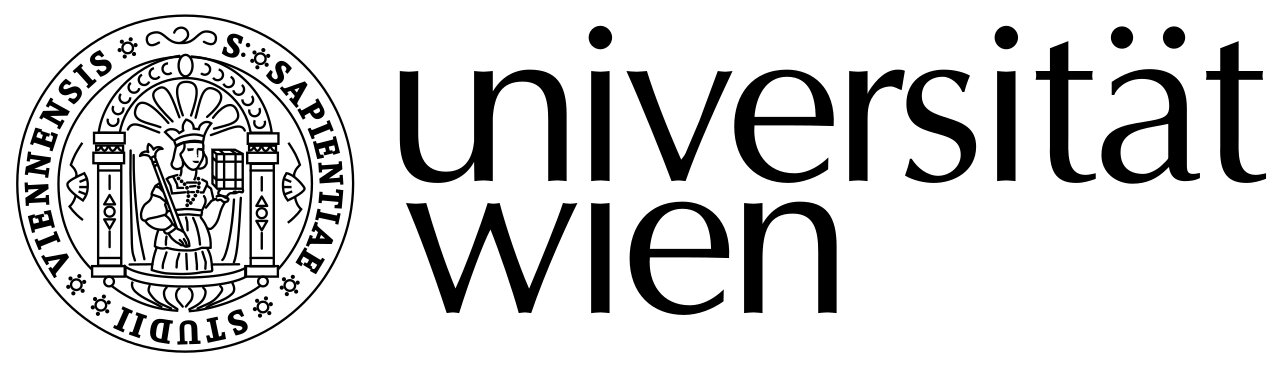
\includegraphics[width=8cm]{logo} \\
%		\Large Fakultät für Mathematik \\
%		\baselineskip=.7cm
		\title{Vorlesungsskript von \textit{Einführung in das mathematische Arbeiten}}
		\author{
%		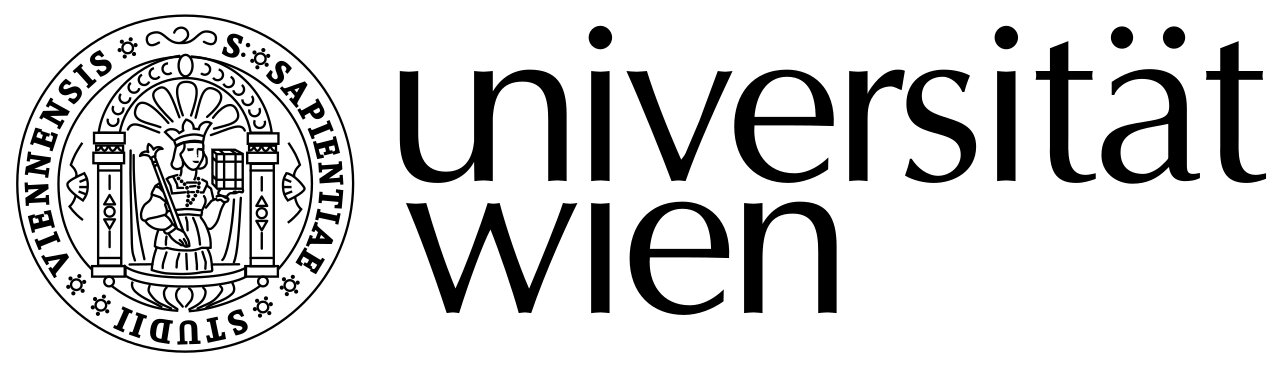
\includegraphics[width=13cm]{logo} \\
		Professor Karlheinz Gröchenig \\ Universität Wien \\ Fakultät für Mathematik}
		
		\date{Wintersemester 2022/2023}
\begin{titlepage}
	\maketitle
	\thispagestyle{empty}
\end{titlepage}
%%%%%%%%%%%%%%%%%%%%%%%%%%%%%%%%%%%%%%%%%%%%%%%%%%%%%%%%%%%%%
%%%%%%%%%%%%%%%%%%%%%%%%%%%%%%%%%%%%%%%%%%%%%%%%%%%%%%%%%%%%%
\newpage
\section[Einleitung und Perspektive]{Einleitung und Perspektive
	\protect\footnote{Einige Teile stammen aus dem Buch "Einführung in das mathematische Arbeiten"}
}
Man kann sich die gesamte Mathematik als ein Gedankengebäude vorstellen, das aus Aussagen besteht. Diese Aussagen bestehen aus anderen Grundaussagen die schon durch logische Schlussfolgerungen abgeleitet werden. Dieser Vorgang heißt \textbf{beweisen}. Gilt eine Aussage $ A $ als bewiesen, und kann man eine weitere Aussage $ B $ logisch aus $ A $ ableiten. Anders ausgedrückt kann man sich einen \textbf{Beweis} als eine Kette logischer Argumente vorstellen, die die Gültigkeit einer mathematischen Aussage sicherstellt. Das Beste ist, sich immer bei einem solcherart logischen Vorgang fragen: welche Teile von den Voraussetzungen berechtigt mich so was zu behaupten?
  
Ein Beispiel von einer mathematischen Aussage:
\begin{center}
		\textit{Das Quadrat einer geraden Zahl ist gerade}
\end{center}
\subsection{Mathematische Begriffe}
Unterschiedliche mathematische Begriffe sind:
\begin{itemize}
	\item \textbf{Satz}
	\item \textbf{Definition}
	\begin{tcolorbox}[colback={white}, colframe={DarkGreen},breakable]
		\begin{definition}\label{11}
			Eine ganze Zahl $ n \in \mathbb{Z} $ heißt \textbf{gerade}, wenn es eine ganze Zahl $ m $ gibt, so dass $ n=m $.
		\end{definition}
	\end{tcolorbox}
	\item \textbf{Proposition}
	\item \textbf{Lemma (Hilfsatz)}
	\begin{tcolorbox}[colback={white}, colframe={DarkGreen},breakable]
		\begin{lem}
			Wenn $ n \in \mathbb{Z} $ gerade ist, dann ist auch $ n^2 $ gerade. (kurzschreibweise: $ 2|n \Rightarrow 2|n^2 $)
		\end{lem}
		\begin{proof}[Beweis (Voraussetzung $\to$ Folgerung)]
			Da $ n $ gerade ist, gibt es $ m \in \mathbb{Z} $ so dass $ n = 2m $. Dann
			\begin{align*}
				n^2 & = (2m)^2 = 4m^2 = 2(\underbrace{2m^2}_{\in \mathbb{Z}}) \xRightarrow[]{\ref{11}} 2 | n^2
			\end{align*}
		\end{proof}
	\begin{proof}[Hinweis]\let\qed\relax
		Wir haben die \textbf{Rechenfolge} für $ \mathbb{Z} $ verwendet:
		\begin{itemize}
			\item $ ab = ba $ \hfill (Kommutativität)
			\item $ (ab)c = a(bc) $ \hfill (Assoziativität) 
		\end{itemize}
	\end{proof}
	\end{tcolorbox}
	\begin{tcolorbox}[colback={white}, colframe={DarkGreen},breakable]
		\begin{lem}
			Ebenso: Das Quadrat einer ungeraden Zahl ist ungerade.
			\begin{proof}
				Bevor wir den Beweis durchgehen, sei darauf hingewiesen, dass "$ n $ ungerade" so heißt: es existiert $ m \in \mathbb{Z} $, so dass $ n = 2m+1 $. Dann
				\begin{align*}
					n^2 = (2m+1)^2 & = 4m^2 + 4m + 1 \\
					& = 2(\underbrace{2m^2 + 2m}_{= m' \in \mathbb{Z}}) + 1 \\
					& = 2m' + 1
				\end{align*}
			\end{proof}
		\end{lem}
	\end{tcolorbox}
	\item \textbf{Wesentlicher Objekt}: Menge der natürlichen Zahlen
	\[ 
	\mathbb{N} = \{ 0,1,2,3,4,\ldots \}
	 \]
	Menge der ganzen Zahlen
	\[ 
	\mathbb{Z} = \{ \ldots , -4 , -3 , -2 , -1 , 0 , 1 , 2 , 3 , 4, \ldots \}
	 \]
	Menge der rationalen Zahlen:
	\[ 
	\mathbb{Q} = \left\{ \frac{m}{n} \mid m,n \in \mathbb{Z}, n \neq 0 \right\}
	 \]
\end{itemize}
\begin{tcolorbox}[breakable]
\subsection*{Eine Denksportaufgabe}
Frau Miller hat drei Töchter: 
\begin{dialogue}
	\speak{Frau Miller} Das Produkt des Alters meiner Töchter ist 36 und die Summe ergibt meine Hausnummer.
	\speak{Nachbarin} Daraus kann ich das Alter der Töchter nicht bestimmen.
	\speak{Frau Miller} Richtig, die älteste spielt Cello.
\end{dialogue}
\noindent Wie alt sind die Töchter?
\begin{lo*}
	Zu Beginn, nehmen wir an, dass Alter eine natürliche Zahl ($ 1,2,3, \ldots  $) ist. Vorgehensweise, schreiben wir mit allen Fallunterscheidungen:
	\[ 
	\begin{array}{cccc}
		&&& \text{Summe} \\
		1 & 1 & 36 & 38 \\
		1 & 2 & 18 & 21 \\
		1 & 3 & 12 & 16 \\
		1 & 4 & 9  & 14 \\
		1 & 6 & 6  & 13 \\
		2 & 2 & 9  & 13 \\
		2 & 3 & 6  & 11 \\
		3 & 3 & 4  & 10
	\end{array}
	\]
	Aus den Daten der Tabelle, kann man herausfinden, dass die Hausnummer 13 ist. sont wäre die Nachbarin eindeutig. Es gibt zwei Auswahlmöglichkeiten, die einer Summe von 13 entsprechen:
	\[ 
	\begin{array}{ccc}
		1 & 6 & 6 \\
		2 & 2 & 9
	\end{array}
	\]
	aber frau Miller hat gesagt: "\textit{Die älteste spielt Cello}". Aber nur in "$ 2 \quad 2 \quad 9 $" gibt es eine explizite Maximalelement. Da es eine älteste Tochter gibt, kommt nur $ (2,2,9) $ als Lösung in Frage.
\end{lo*}
\end{tcolorbox}
\newpage
\section{Zahlentheorie}
\begin{definition}[Teilbarkeit]
	Sei $ n \in \mathbb{Z} $:
	\begin{enumerate}
		\item $ d \in \mathbb{Z} $ heißt \textbf{teilbar von $ \mathbf{m} $}, wenn es $ m \in \mathbb{Z} $ gibt, so dass $ n = dm $. (Schreibweise: $ d|n $ bedeutet: $ \exists m \in \mathbb{Z}: n=dm $)
		\item 
		$ n $ heißt Primzahl, wenn $ \pm 1 $ und $ \pm n $ die einzige Teiler von $ n $ sind und $ n > 1 $.
	\end{enumerate}
\end{definition}
\begin{definition}
	$ \mathbb{P} $ ist die Menge der Primzahlen und ist eine Teilmenge von $ \mathbb{N} $.
\end{definition}
\begin{bei*}
	\[ 
	\begin{array}{lll}
		2|n & & n \,\, \text{gerade} \\
		2|10 & 5|10 & \\
		3 \not| 10 & & 3 \,\, \text{ist kein Teiler von} \,\, 10	
	\end{array}
	 \]
\end{bei*}
\begin{lem}
	Seien $ d,m,n \in \mathbb{Z} $ wenn $ d|m $ und $ d|n $ dann gilt auch $ d|m+n $.
\end{lem}
\begin{proof}
	Nach Voraussetzung gibt es $ k,l \in \mathbb{Z} $, so dass $ m = kd $ und $ n = ld $. Dann ist 
	$ m+n = kd + ld = (k+l)d $. Da $ k+l \in \mathbb{Z} $ gilt $ d|m+n $.
\end{proof}
\begin{bem}[Wohlordnung von $ \mathbb{N} $] \label{12}
	Jede Menge von natürlichen Zahlen hat ein kleinstes Element.
\end{bem}
\begin{sa}[Primzahlzerlegung der natürlichen Zahlen]\label{21}
	Sei $ n \in \mathbb{N} $, $ n>1 $ dann gibt es endlich viele Primzahlen (nicht notwendigerweise verschieden) $ P_1 , P_2 , \ldots , P_n $ sodass $ n = P_1 P_2 \cdots P_n $.
\end{sa}

\begin{proof}
	Versuchen wir indirekten Beweis. Angenommen Behauptung stimmt nicht; wir müssen ein Widerspruch herleiten (Wenn ein Widerspruch abgeleitet wird, bedeutet das, dass aus $ \neg B $, $ \neg A $ das Ergebnis ist und das bedeutet, dass $ \neg B \Rightarrow \neg A $ und damit sein Äquivalent $ A \Rightarrow B $ wahr ist). Angenommen, es gilt $ n \in \mathbb{N} $ sodass sich $ n $ nicht als Produkt von endlich vielen Primzahlen schneiden lässt. Dann gilt es ein kleinstes $ n \in \mathbb{N} $. Beachten Sie, dass es eine Eigenschaft von der Menge der natürlichen Zahlen (\ref{12}) ist. 
	\begin{proof}[Fall 1]\let\qed\relax
		$ n $ ist eine Primzahl, dann ist n bereits Produkt aus Primzahlen. Angenommen $ n = P_1 $ und $ P_1 $ ist eine Primzahl. Dann können wir schreiben:
		\[ 
		n = \prod\limits_{k=1}^1 P_k
		 \]	
		also $ n $ ist Produkt aus Primzahlen.
	\end{proof}
	\begin{proof}[Fall 2]\let\qed\relax
		$ n $ ist keine Primzahl. Dann besitzt $ n $ einem Teiler $ d $ und $ d|n $. es gibt also $ m \in \mathbb{N} $, so dass $ n = d\cdot m $. Da $ m = \frac{n}{d} $, gilt $ 1 < m < n $. \\
		Da $ d < n $ und $ m<n $, lassen sich $ d $ und $ m $ als Produkt von Primzahlen schneiden. Als
		$ d = q_1 q_2 \cdots q_k $ und $ m = r_1 r_2 \cdots r_l $ dann insgesamt ist die Zahl $ n = md $ selbstverstätndlich hergestellt von endlich vielen Primzahlen. Es ist ein Widerspruch zur Eigenschaft von $ n $, die wir schon angenommen haben.
	\end{proof}
\end{proof}
\begin{sa}
	Es gibt unendlich viele Primzahlen.
\end{sa}
\begin{proof}[Ein indirekter Beweis]
	Angenommen Behauptung stimmt nicht. Bilde die Zahl $ m = p_1 \cdots p_n + 1 $. Nach Satz \ref{21} lässt sich $ m $ als Produkt von Primzahlen schneiden. Insbesonders gibt es eine Primzahl die $ m $ teilt. Diese Primzahl kommt unter den Primzahlen $ P_1 ,P_2, \ldots , P_n $ vor, also gibt es $ P_j $ so dass $ P_j | m $. Dann gilt einerseits $ P_j | m $ und anderseits $ P_j | P_1P_2\cdots P_n $. Dann gilt $ P_j | m - (P_1P_2 \cdots P_n) $. Dann gilt $ P_j | 1 $ und das heißt, dass es eine Zahl $ m $ in der natürlichen Menge gibt, so dass $ 1 = P_j m $. Dann $ 0 < m = \frac{1}{P_j} < 1 $ und das ist ein Widerspruch. Denn $ m $ ist eine natürliche Zahl und kann nicht kleiner als $ 1 $ sein. 
\end{proof}
\begin{bem}
	Die Menge der rationale Zahlen ist
	$ \mathbb{Q} = \{ \frac{m}{n} \mid m,n \in \mathbb{Z}, n \neq 0 \} $. Durch Kürzen können wir immer annehmen, dass $ m $ und $ n $ keinen echten gemeinsamen Teiler besitzen. Dass heißt falls 
	$ d|m $ und $ d|n $, gilt $ d = \pm 1 $ und falls $ m=dh $, $ n=dl $ und $ d \neq \pm 1 $, gilt 
	$ \frac{m}{n} = \frac{dh}{dl} = \frac{h}{l} $.
\end{bem}
\begin{sa}
	$\sqrt{2} \notin \mathbb{Q} $ ($ \sqrt{2} $ ist irrational).
\end{sa}
\begin{proof}
	Angenommen $ \sqrt{2} $ ist rational. D.h. es gibt $ m,n \in \mathbb{N} $, so dass $ \sqrt{2} = \frac{m}{n} $. Dann gilt $ 2 = \frac{m^2}{n^2} $ oder $ m^2 = 2n^2 $. Dann ist $ m^2 $ gerade, daher ist auch $ m $ gerade. Dann gibt es $ k \in \mathbb{N} $ so dass $ m = 2k $. Dann gilt
	\[ 
	m^2 = (2k)^2 = 2\cdot 2k^2 = 2n^2
	 \]
	 und Kürzen liefert $ n^2 = 2k^2 $. Daher muss wieder $ n $ gerade sein. Also $ n = 2l $ für ein 
	 $ l \in \mathbb{N} $. $ m = 2k $ und $ n = 2l $ heißt $ 2 $ ist ein gemeinsamer Teiler von $ m $ und $ n $. Widerspruch zur Wahl von $ m $ und $ n $.
\end{proof}
\begin{sa}[Division mit Rest]
	Sei $ a \in \mathbb{Z} $, $ n \in \mathbb{N} $ und $ n \neq 0 $, Dann gibt es eindeutige $ q,r \in \mathbb{Z}, 0 \leq r \leq n $ so dass $ a = qn + r $.
\end{sa}
\begin{proof}[Beweis von Existenz]
	Betrachte die Menge S als
	\begin{align*}
		S & = \{ \ldots , a - n , a , a + n , a + 2n , \ldots \} \cap \mathbb{N} \\
		& = \{ m = a+qn : q \in \mathbb{Z} \} \cap \mathbb{N}
	\end{align*}
	Da $ S \subseteq \mathbb{N} $, gibt es ein kleinstes Element $ r $ in $ S $. Es gibt
	\begin{itemize}
		\item $ n \geq 0 $
		\item $ r = a - qn $ für ein $ q \in \mathbb{Z} $ also $ a = qn+r $
		\item $ r < n $. falls $ r \geq n $ wäre, gilt
		\[ 
		a - (q+1)n = \underbrace{a-qn-n}_{\in S} = r-n \geq 0
		 \]
		und das ist ein Widerspruch zu der Annahme, die $ r $ als das kleinste Element beurteilt. Weil $ a-qn-n $, ein positives Element der Menge S und kleiner als $ r $ ist. Dann $ r < n $.
	\end{itemize}
\end{proof}
\end{document}